\documentclass[10pt,a4paper]{article}

\usepackage{float}

\usepackage{hyperref}

\usepackage{graphicx}

\usepackage {bsymb,b2latex}
\usepackage[utf8]{inputenc}
\usepackage{fancyhdr,lastpage,color}
\pagestyle{plain}
%---------------------------------------------------------

\newcommand{\true}{\ensuremath{true}}
\newcommand{\btext}[1]{{\it #1}}
\newcommand{\bvar}[1]{\btext{#1}}
\newcommand{\bevent}[1]{\btext{#1}}
\newcommand{\binv}[1]{\btext{#1}}
\newcommand{\bconst}[1]{\btext{#1}}
\newcommand{\bparam}[1]{\btext{#1}}
\newcommand{\bfunc}[1]{\btext{#1}}
\newcommand{\baxiom}[1]{\btext{#1}}
\newcommand{\btype}[1]{\btext{#1}}
\newcommand{\bguard}[1]{\btext{#1}}

% scaling for project creation wizard screenshots
\newcommand{\skalierung}{.6}

\title{Using Rodin with Projects on github}

\author{Systerel, France}

\date{}

\begin{document}

\maketitle

\begin{abstract}
  This document explains how Rodin projects on github can be imported into the
  Rodin platform. This is illustrated using the \texttt{model-evaluation}
  sub-project of \texttt{openETCS}.
\end{abstract}

\section{Prerequisites}
\label{sec:prerequisites}

This section shortly describes the basic prerequisites to use Rodin projects on
github. First the installation of the Rodin platform itself, then the basic
plugins required to use the provided models and finally additional plugins which
facilitate usage and extension of the provided models.

\subsection{Rodin Platform}
\label{sec:rodin-platform}

This illustration uses the Rodin platform
2.7~\footnote{\url{http://www.event-b.org/}}, for general information on
Event-B, Rodin, various plugins etc. see the Event-B
Wiki~\footnote{\url{http://wiki.event-b.org/index.php/Main_Page}}. More details
on the installation on Rodin can be found
at {\url{http://www.event-b.org/install.html}}.

\subsection{Basic Plugins}
\label{sec:basic-plugins}

For plugin installations, it is recommended to tick the ``Contact all update
sites during install to fin required software'' (see
Figure~\ref{fig:plugin-install}). This will install all necessary dependencies
for each plugin, in case these are not yet installed.

\begin{figure}[ht]
  \centering
  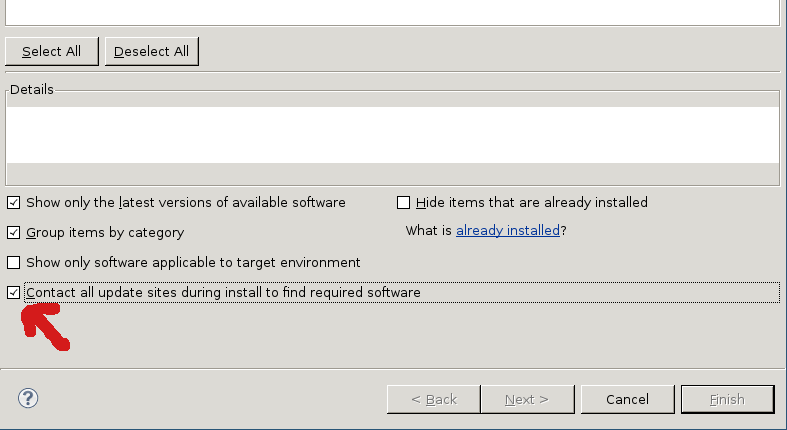
\includegraphics[width=.75\textwidth]{install-plugin}
  \caption{Plugin Installation}
  \label{fig:plugin-install}
\end{figure}

\paragraph{Atelier-B Provers}
\label{sec:atelier-b-provers}

The Atelier-B provers facilitate the construction of the proof trees for Rodin
proof obligations, by automatically discharging may proof obligations. Their
repository is available under Rodin as ``Atelier B Provers''.

\paragraph{ProR Integration}
\label{sec:pror-integration}

The integration with ProR allows for the traceability of requirements in the
provided ReqIf files. The repository is available under Rodin as ``ProR'', where
the ``ProR Rodin integration feature'' must be installed. {\bf NOTE: } For the
current ProR version 0.6.0 there are known problems with Java version 6. It is
suggested to use Java version 7, if possible the latest JVM from
\url{http://www.oracle.com/technetwork/java/javase/downloads/jdk7-downloads-1880260.html}.

\paragraph{EGit}
\label{sec:egit}

The integration with github is done via the EGit plugin. This plugin allows to
collaborate on Rodin models and to push/pull changes to github. The repository
is available under the official Eclipse repositories as ``Indigo Update Site''
where the ``Eclipse EGit'' must be installed.

\subsection{Additional Plugins}
\label{sec:additional-plugins}

The additional plugins are not strictly necessary to analyze and inspect the
model. Nevertheless, it is suggested to install them if an extension of the
model is intended.

\paragraph{ProB}
\label{sec:prob}

The ProB plugin provides means for model-checking and animation of Event-B
models. This requires finite instantiation of carrier sets and selection of an
initial state. In this situation, the plugin can verify deadlock freeness and
LTL formulas or can animate a system run. It is available from the ProB
repository under ``ProB for Rodin 2''.

\paragraph{SMT Solver Plugin}
\label{sec:smt-solver-plugin}

The SMT solver plugin will in general lead to a higher degree of automation for
the formal proofs. Experiments with industrial cases studies reduced the number
of non-automatically discharged proof obligations to one fourth. The plugin
comes bundled with two different solvers (CVC3 and veriT) and it can be extended
with various other, e.g., z3 from Microsoft or MathSAT5 from FBK. It is
available from the Rodin repository under ``SMT Solvers Integration''.

\paragraph{iUML-B State Machines}
\label{sec:iuml-b-state}

The ``iUML-B State-Machines'' plugin allows for graphical modeling of
state-machines in an Event-B model. The state machines can be transformed into
Event-B code. It has a good integration with the ProB plugin which allows for
graphical animation of the machines.

\paragraph{Project Diagram}
\label{sec:project-diagram}

The project diagram plugin allows for visualization of the structure of a
model. In particular it visualizes the refinement relations between the
machines, the extension relation between the contexts and the sees relation
between machines and contexts. It is available from the Rodin repository under
``Event-B Project Diagram Plugin''.

\section{Importing Rodin Projects from github}
\label{sec:import-rodin-proj}

After the installation of Rodin and the necessary plugins, projects can be
imported from github into the local Rodin workspace. In the following, this is
explained using the Eclipse project creation wizard.

The first step is to select ``File $\rightarrow$ New $\rightarrow$ Event-B
Project'' from the Eclipse menu and then to select ``Git $\rightarrow$ Projects
from Git'' as import source (see Figure~\ref{fig:create-new-project}).

\begin{figure}[H]
  \centering
  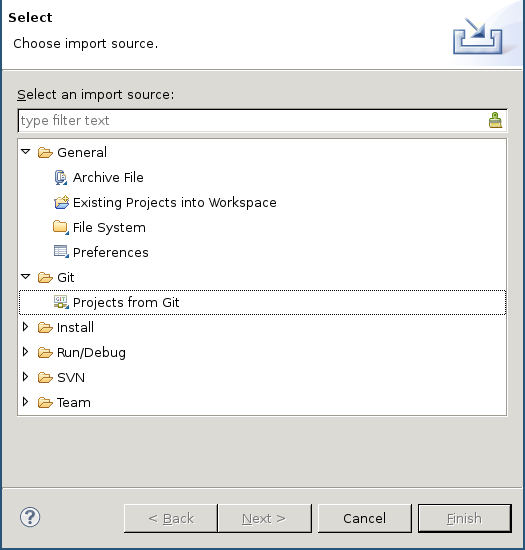
\includegraphics[width=\skalierung\textwidth]{project_import_step1}
  \caption{Creating a New Project}
  \label{fig:create-new-project}
\end{figure}

The next step is to specify where to find the git repository. For this, one has
to select the URI option as shown in Figure~\ref{fig:select-repo-source}.

\begin{figure}[H]
  \centering
  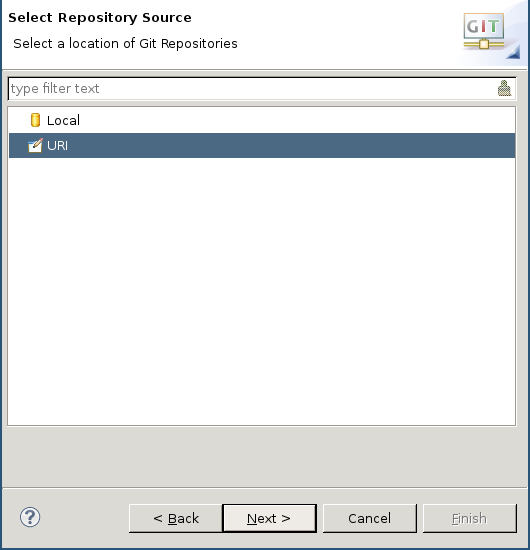
\includegraphics[width=\skalierung\textwidth]{project_import_step2}
  \caption{Selection of Repository Source}
  \label{fig:select-repo-source}
\end{figure}

The next step is to specify the URI of the repository on github. For the
model evaluation project, this is
\url{https://github.com/openETCS/model-evaluation.git}. This step also requires
the specification of the authentication data, i.e., the username and password
for github (see Figure~\ref{fig:specify-git-repo}).

\begin{figure}[H]
  \centering
  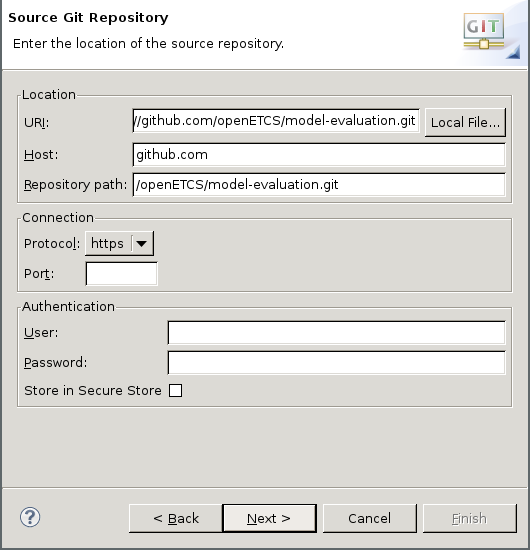
\includegraphics[width=\skalierung\textwidth]{project_import_step3}
  \caption{Specify github Repository}
  \label{fig:specify-git-repo}
\end{figure}

The next step is to select the desired branch of the repository. If in doubt and
there is more than one branch, selecting the ``master'' branch, as shown in
Figure~\ref{fig:select-branch} should be ok.

\begin{figure}[H]
  \centering
  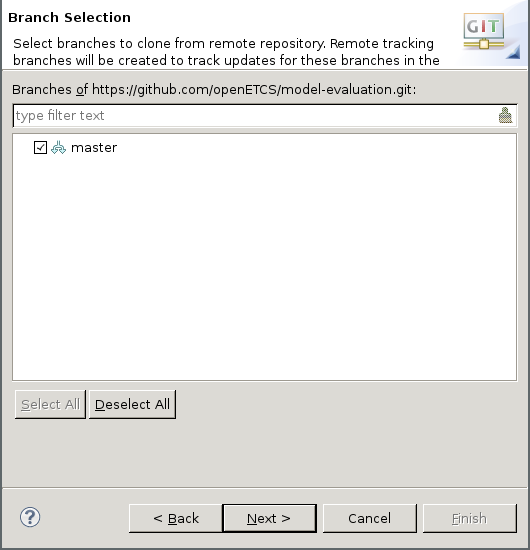
\includegraphics[width=\skalierung\textwidth]{project_import_step4}
  \caption{Select Branch of Repository}
  \label{fig:select-branch}
\end{figure}

For a local copy of the repository on github, an empty directory on the local
machine must be selected (or created) and a name of the remote repository can be
specified, the default is ``origin'' (see Figure~\ref{fig:local-copy}).

\begin{figure}[H]
  \centering
  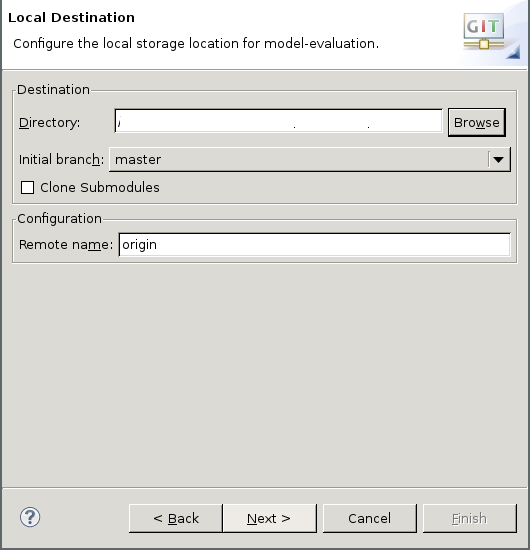
\includegraphics[width=\skalierung\textwidth]{project_import_step5}
  \caption{Local Repository Copy}
  \label{fig:local-copy}
\end{figure}

As there can be multiple projects in a repository, e.g., from different tools as
for the model-evaluation project, the correct one must be selected. To achieve
this, the collapsed directory tree as shown in
Figure~\ref{fig:select-project-import} must be expanded\footnote{Sometimes the
  information which directories are available is not shown directly (the
  collapse / expand symbol is lacking besides the ``working directory''). In
  this case it helps to push the ``back'' button to the previous window and
  return with ``next''.}.

\begin{figure}[H]
  \centering
  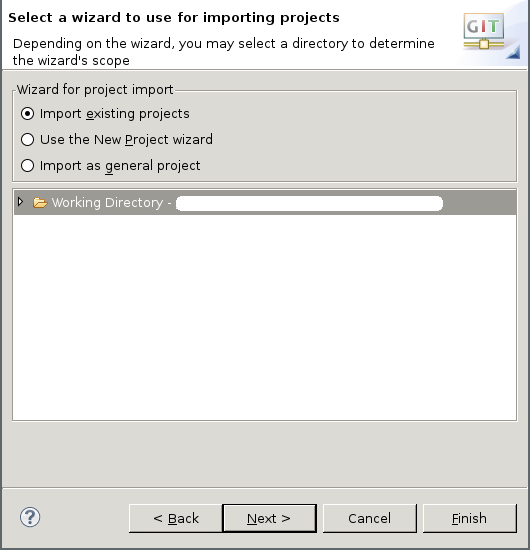
\includegraphics[width=\skalierung\textwidth]{project_import_step6}
  \caption{Select Project to Import}
  \label{fig:select-project-import}
\end{figure}

In the expanded tree, the project root directory of the project must be selected
as shown in Figure~\ref{fig:expanded-tree}.

\begin{figure}[H]
  \centering
  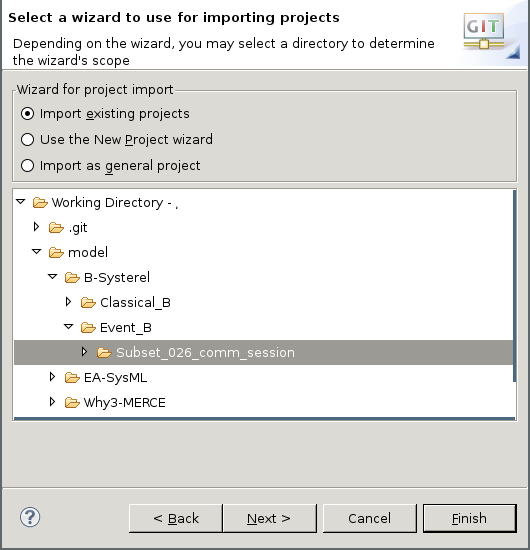
\includegraphics[width=\skalierung\textwidth]{project_import_step7}
  \caption{Expanded Directory Tree}
  \label{fig:expanded-tree}
\end{figure}

Once the correct directory has been selected, the contained projects can be
selected as shown in Figure~\ref{fig:import-project-workspace} and imported into
the local Rodin workspace.

\begin{figure}[H]
  \centering
  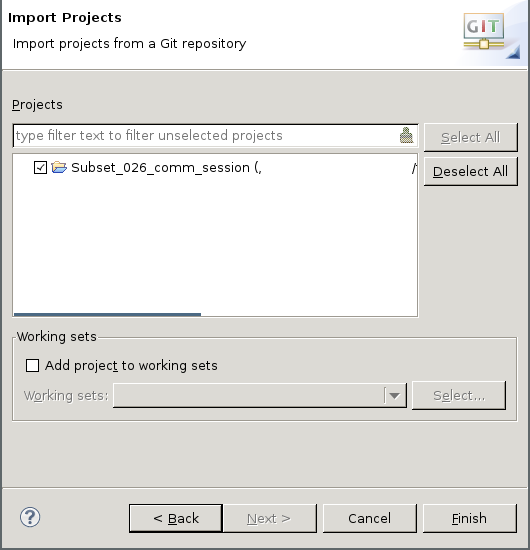
\includegraphics[width=\skalierung\textwidth]{project_import_step8}
  \caption{Import Project into Workspace}
  \label{fig:import-project-workspace}
\end{figure}

\section{Frequently Asked Questions - FAQ}
\label{sec:faq}

\begin{itemize}
\item {\bf How are requirements traced?}

  For requirements tracing we use the ProR
  plugin~\footnote{http://wiki.event-b.org/index.php/ProR} from
  formalmind~\footnote{http://www.formalmind.com}. It is based on the OMG
  standardized ReqIf format. It allows for tracing of Event-B modeling artifacts
  in ReqIf files. Changes in either the model or the ReqIf are marked
  automatically, the ProR view of Rodin is shown in
  Figure~\ref{fig:req-tracing}.


  \begin{figure}[H]
    \centering
    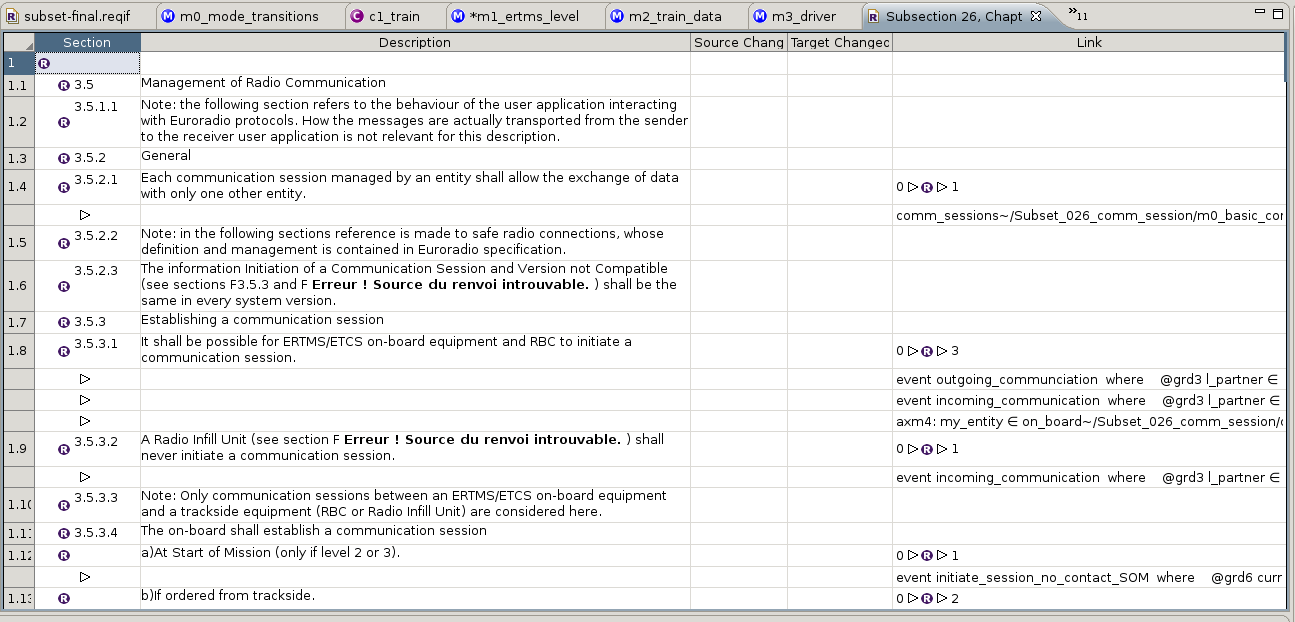
\includegraphics[width=\textwidth]{ReqIfinRodin}
    \caption{Requirements Tracing with ProR}
    \label{fig:req-tracing}
  \end{figure}

  To open a ReqIf file, the ``Resources'' view of Rodin must be selected which
  will show all files in the project in the Project-Explorer.

\item {\bf Proof obligations are not shown in the Event-b explorer. How to
    create them?}

  This can have different causes. Trivial proof obligations are not shown, this
  concerns in particular proofs for well-definedness~\footnote{see
    \url{http://handbook.event-b.org/current/html/well_definedness_proof_obligations.html}}. It
  is also possible to hide proven proof obligations by toggling the green button
  on top of the Event-B Explorer shown in
  Figure~\ref{fig:tree-proof-obligations} (button is inactive in this example).

  \begin{figure}[H]
    \centering
    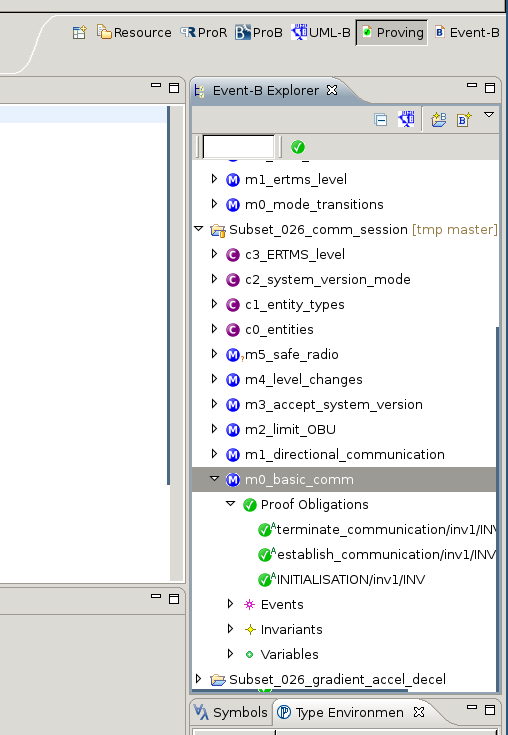
\includegraphics[width=.5\textwidth]{RodinEventBView}
    \caption{Event-B Project Tree View with Proof Obligations}
    \label{fig:tree-proof-obligations}
  \end{figure}

  Another possibility is a problem with some installed plugins, in this case the
  project can be cleaned by selecting ``Project->Clean'' from the main Rodin
  menu. If  ``Project->Build Automatically'' is selected the project will be
  automatically refreshed, this is also possible manually by selecting the
  project, hitting F5 or selecting ``Refresh'' from the right-click menu.

\item {\bf If I try to open a ReqIf file, Rodin nothing happens and Rodin
    freezes. What happened?}

  There is a problem in the ProR plugin which can cause this behavior (e.g., see
  here \url{https://bugs.eclipse.org/bugs/show_bug.cgi?id=397672}). Currently
  the best solution is to install the most recent JDK
  from~\url{http://www.oracle.com/technetwork/java/javase/downloads/jdk7-downloads-1880260.html}.

\end{itemize}

\end{document}




%%% Local Variables:
%%% mode: latex
%%% TeX-master: t
%%% End:
